In this section we first motivate the need for LRCCA by exploring the performance of RCCA
for various regularization parameters. We then explore the accuracy of Theorem
\ref{thm:xy_sv}. While this theorem gives an asymptotic limit, we show that the
finite-sized approximation holds for moderately sized systems. 

For all of the following simulations, we generate correlated signal datasets by
\be\ba
&\widetilde{X}^{\text{signal}} = \left[\widetilde{x}_1^{\text{signal}},\dots,\widetilde{x}_n^{\text{signal}}\right]\\
&\widetilde{Y}^{\text{signal}} = \left[\widetilde{x}_1^{\text{signal}},\dots,\widetilde{y}_n^{\text{signal}}\right]
\ea\ee
where
\be\ba
&\widetilde{x}_i^{\text{signal}} = U_x\Theta_xv_x^{(i)} + x_i\\
&\widetilde{y}_i^{\text{signal}} = U_y\Theta_yv_y^{(i)} + y_i,
\ea\ee
where $x_i\sim\mathcal{N}(0,I_p)$ and $y_i\sim\mathcal{N}(0,I_q)$ and
\be 
\left[\begin{array}{c}v_x^{(i)}\\v_y^{(i)}\end{array}\right]
\sim\mathcal{N}\left(\left[\begin{array}{cc}I_r &P\\P^T &I_r \end{array}\right]\right).
\ee
$P=\diag(\rho_1,\dots,\rho_r)$ with $0\leq\rho_i\leq1$ and
$\Theta_x=\diag(\theta_{x1},\dots,\theta_{xr})$ and
$\Theta_y=\diag(\theta_{y1},\dots,\theta_{yr})$ with $\theta_{xi}\geq0$ and
$\theta_{yi}\geq0$. We generate $U_x$ by taking the eigenvectors corresponding to the top
$r$ eigenvalues of a random $p\times p$ matrix with $\mathcal{N}(0,1)$ entries. We
generate $U_y$ independently in a similar manner. 

We then generate noise only datasets
\be\ba
&\widetilde{X}^{\text{noise}} =
\left[\widetilde{x}_1^{\text{noise}},\dots,\widetilde{x}_n^{\text{noise}}\right]\\ 
&\widetilde{Y}^{\text{noise}} =
\left[\widetilde{x}_1^{\text{noise}},\dots,\widetilde{y}_n^{\text{noise}}\right] 
\ea\ee
where
\be\ba
&\widetilde{x}_i^{\text{noise}} \sim\mathcal{N}(0,I_p)\\
&\widetilde{y}_i^{\text{noise}} \sim\mathcal{N}(0,I_q).
\ea\ee

\subsection{Performance of RCCA}

First we explore the effect of the regularization parameter in RCCA. For the above simulation
setup we generate both correlated signal data matrices and
with $r=1$ and noise only data matrices. We are interested the distribution of the
correlation estimate, $\widehat{\rho}$, returned by RCCA when there is a correlation present
($\widetilde{X}^{\text{signal}}$ and $\widetilde{Y}^{\text{signal}}$), and when there is no
correlation present ($\widetilde{X}^{\text{noise}}$ and
$\widetilde{Y}^{\text{noise}}$). 

For a fixed $p=100$, $q=150$, and $\rho_1=0.9$ we compute this RCCA correlation estimate
under each hypothesis for 500 trials giving
$\left[\widehat{\rho}_1^{\text{signal}},\dots,\widehat{\rho}_{500}^{\text{signal}}\right]$
and
$\left[\widehat{\rho}_1^{\text{noise}},\dots,\widehat{\rho}_{500}^{\text{noise}}\right]$. We
then compute the empirical ROC (receiver operating characteristic) curve for these two
statistics and the resulting AUC (area under the ROC curve). We repeat this process by
varying $\theta=\theta_{x1}=\theta_{y1}$ and $n$. We plot AUC heatmaps for four different
values of the RCCA regularization parameter in Figure \ref{fig:chpt6:rcca}. AUC values close to
0.5 indicate the distributions of $\widehat{\rho}^{\text{signal}}$ and
$\widehat{\rho}^{\text{noise}}$ are not separable while values close to 1 indicate that
they are perfectly separable. 

As evident in this figure, the ability of RCCA to detect the presence of a signal increases
with the regularization parameter. This is a non-intuitive result as typical regularized
algorithms` have an optimal regularization parameter that maximizes performance. The
non-monotonicity of the AUC heatmaps evident in Figures \ref{fig:chpt6:rcca1} and
\ref{fig:chpt6:rcca2} also give credence to the difficulty in selecting an appropriate
regularization parameter. In certain regimes, increasing the number of samples reduces
performance, which is a very undesirable property. Based on these empirical observations
about the effect of the regularization parameter in RCCA, we conclude that setting
$\eta\to\infty$ results in optimal performance of RCCA. As is stated in Theorem
\ref{thm:lrcca}, in this regime the solution RCCA is found by simply taking the SVD of
$\frac{1}{n}\widetilde{X}\widetilde{Y}^T$. 

\begin{figure}[h!]
  \centering
  \subfigure[$\eta=0.0001$]{
    \label{fig:chpt6:rcca1}
    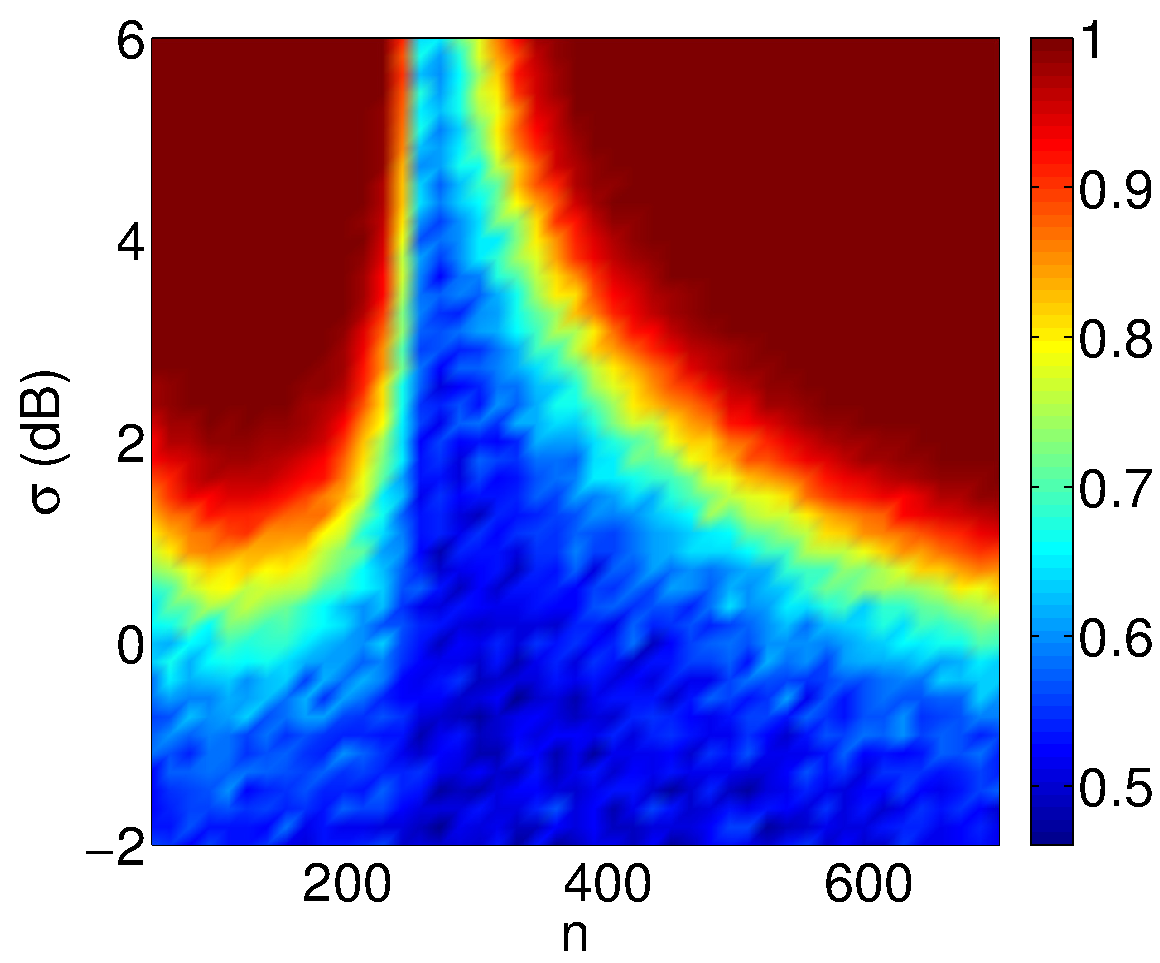
\includegraphics[width=0.4\textwidth]{chpt6_xy/figures/eta1_auc.pdf}
  }
  \subfigure[$\eta=0.1$]{
    \label{fig:chpt6:rcca2}
    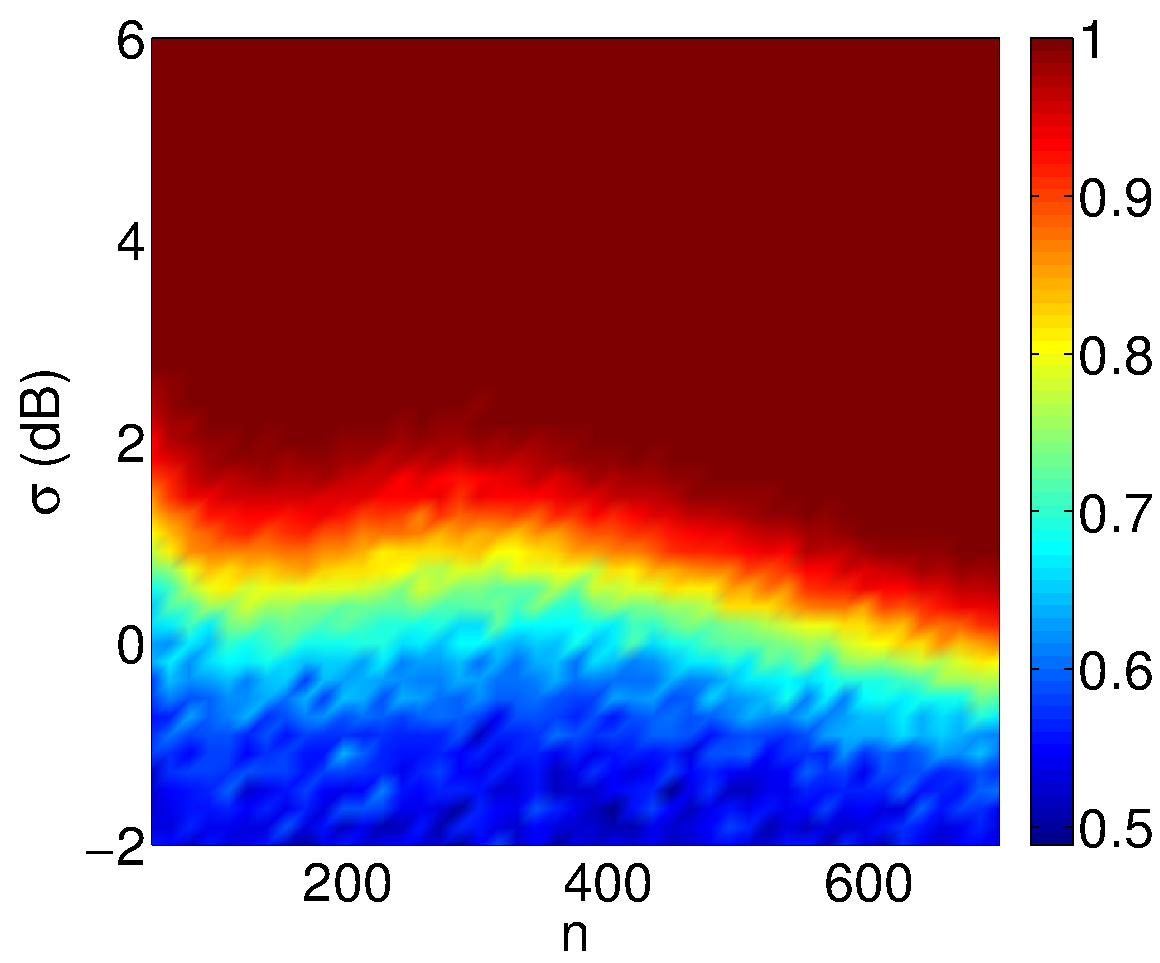
\includegraphics[width=0.4\textwidth]{chpt6_xy/figures/eta2_auc.pdf}
  }
  \subfigure[$\eta=10$]{
    \label{fig:chpt6:rcca3}
   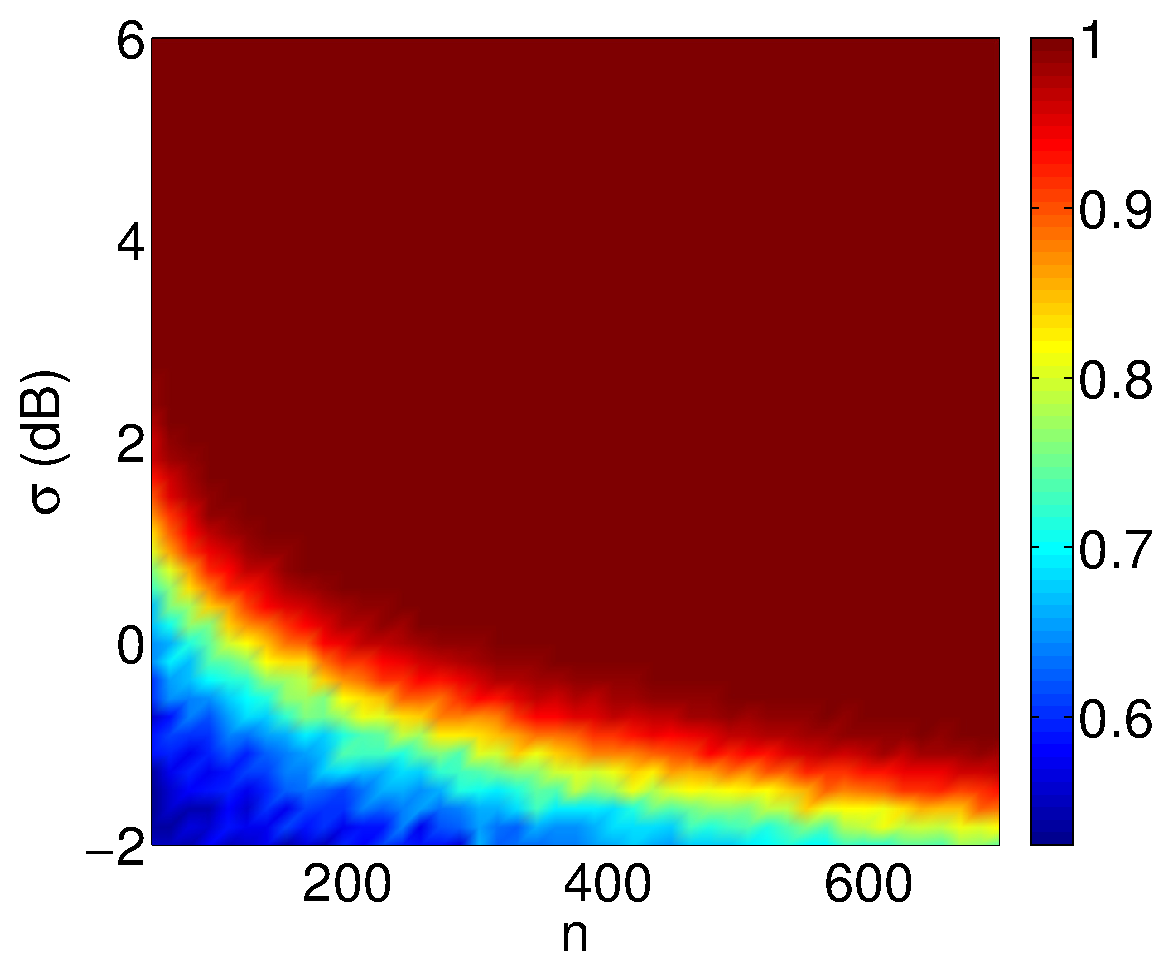
\includegraphics[width=0.4\textwidth]{chpt6_xy/figures/eta3_auc.pdf}
  }
  \subfigure[$\eta=1000$]{
    \label{fig:chpt6:rcca4}
    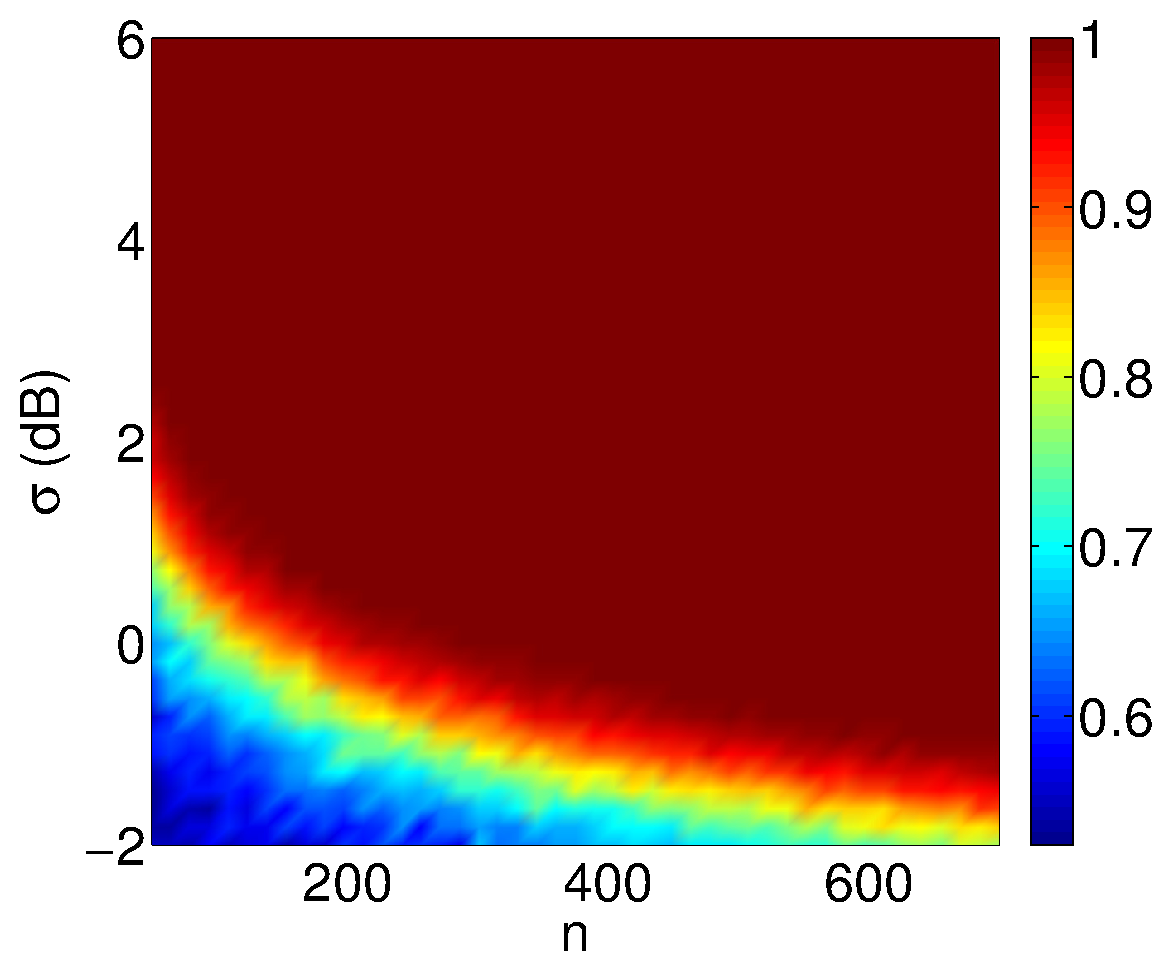
\includegraphics[width=0.4\textwidth]{chpt6_xy/figures/eta4_auc.pdf}
  }
  \caption{AUC performance of RCCA for various regularization parameters. For all figures, $p=100$,
    $q=150$, $r=1$, and $\rho_1=0.9$. Each figure plots an AUC heatmap while sweeping over
  $\theta=\theta_{x1}=\theta_{y1}$ and $n$. AUC points are generated from an ROC formed
  from 500 points of each distribution. Increasing the regularization parameter increases
  the performance of CCA. This gives rise to LRCCA, which sets $\eta\to\infty$.}
  \label{fig:chpt6:rcca}
\end{figure}

\subsection{Numerical Accuracy of Theorem \ref{thm:xy_sv}}

For $p=200$, $q=400$, $n=400$, and $\rho=1$ we compute the largest singular value returned
by LRCCA for various $\theta=\theta_{x1}=\theta_{y1}$. This is repeated and for 100 trials
and compared to the theoretical prediction. Results are shown in Figure \ref{fig:chpt6:sv_pred}
and confirm the accuracy of our theoretical prediction. As evident in Figure
\ref{fig:chpt6:sv_pred}, if $\theta$ is below a critical value, the largest singular value does
not change and remains constant. This phase transition phenomenon arises in similar
analyses of eigenvalue decomposition and SVDs of signal-plus-noise models \cite{benaych2011eigenvalues,benaych2012singular,paul2007asymptotics}. This limiting value is the largest singular value of the noise matrix
$\frac{1}{n}XY^T$, which we define as $b=\sigma_1\left(XY^T\right)$. Substituting $b$ into
(\ref{eq:thm}) we have the following equality
\beq\label{eq:pt}
 0=\left(\varphi_H(b)\varphi_F(b) -
\frac{1}{\theta_{y1}^2}\right)\left(\varphi_J(b)\varphi_G(b) -
\frac{1}{\theta_{x1}^2}\right) -
\rho\varphi_H(b)\varphi_G(b)\left(1+\varphi_K(b)\right)^2.
\eeq
This equation may be solved for any desired parameter $c_x, c_y, \theta_{x1}, \theta_{y1},
\rho$, while keeping the rest fixed. We note that the $\varphi$ functions and $b$ are implicitly dependent on $c_x$ and $c_y$.

\begin{figure}
  \begin{center}
    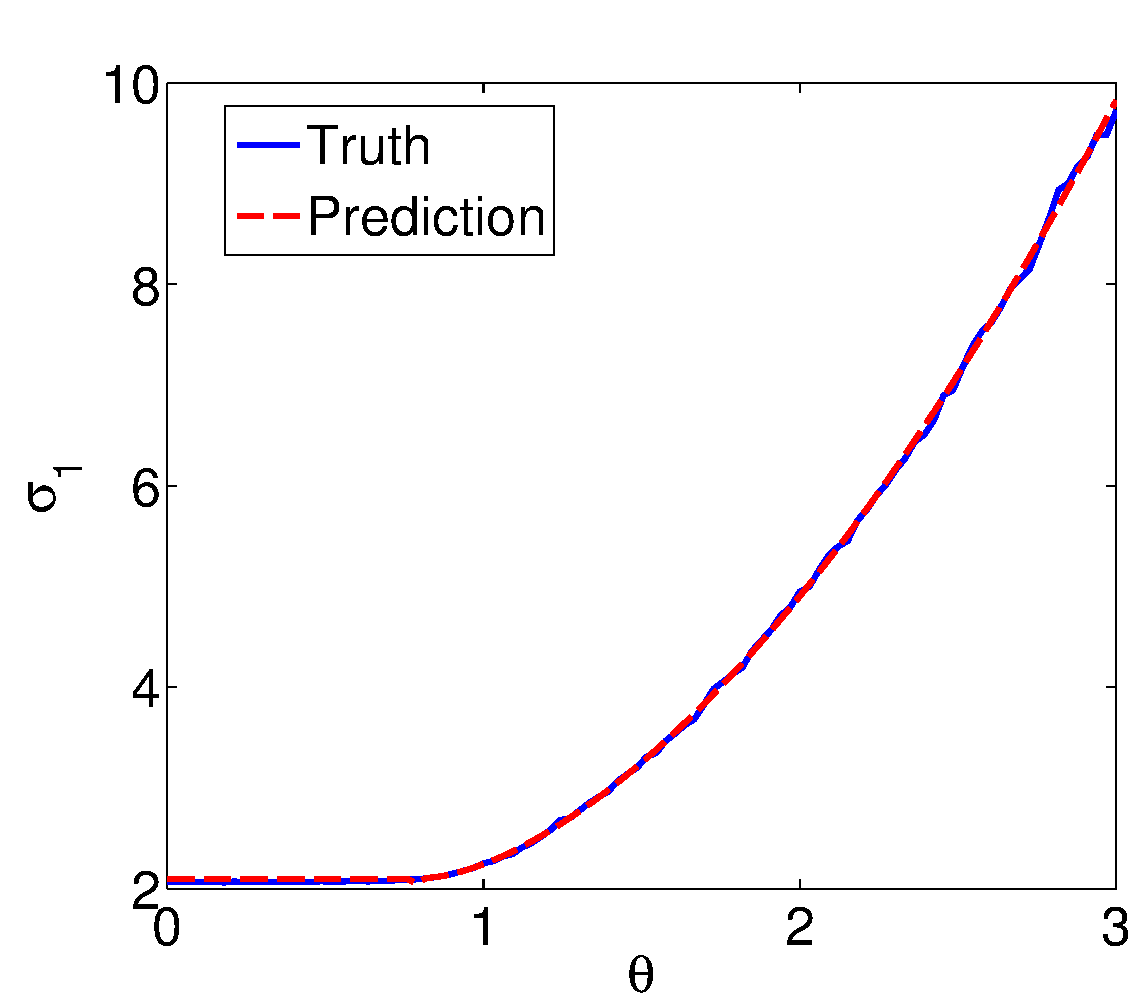
\includegraphics[width=0.6\textwidth]{chpt6_xy/figures/sigma_pred.pdf}
    \caption{Top singular value prediction for the rank-1 case for $p=200$, $q=400$,
      $n=400$, and $\rho=1$.}
    \label{fig:chpt6:sv_pred}
  \end{center}
\end{figure}

Figure \ref{fig:chpt6:lrcca_pt} plots the top singular value returned by LRCCA when the datasets
contain $r=1$ signal each, empirically averaged over 500 trials. Each heatmap sweeps over
two parameters while keeping the rest constant. We then solve (\ref{eq:pt}) by
substituting our constant parameters to achieve a function of the two parameters that we
sweep. We overlay this line in each heatmap. Below this line the
top singular value is indistinguishable from that returned by LRCCA with noise only
datasets.

\begin{figure}[!htbp]
  \centering
  \subfigure[$\rho=1$, $\theta=\theta_{x1}=\theta_{y1}$]{
    \label{fig:chpt6:rcca1}
    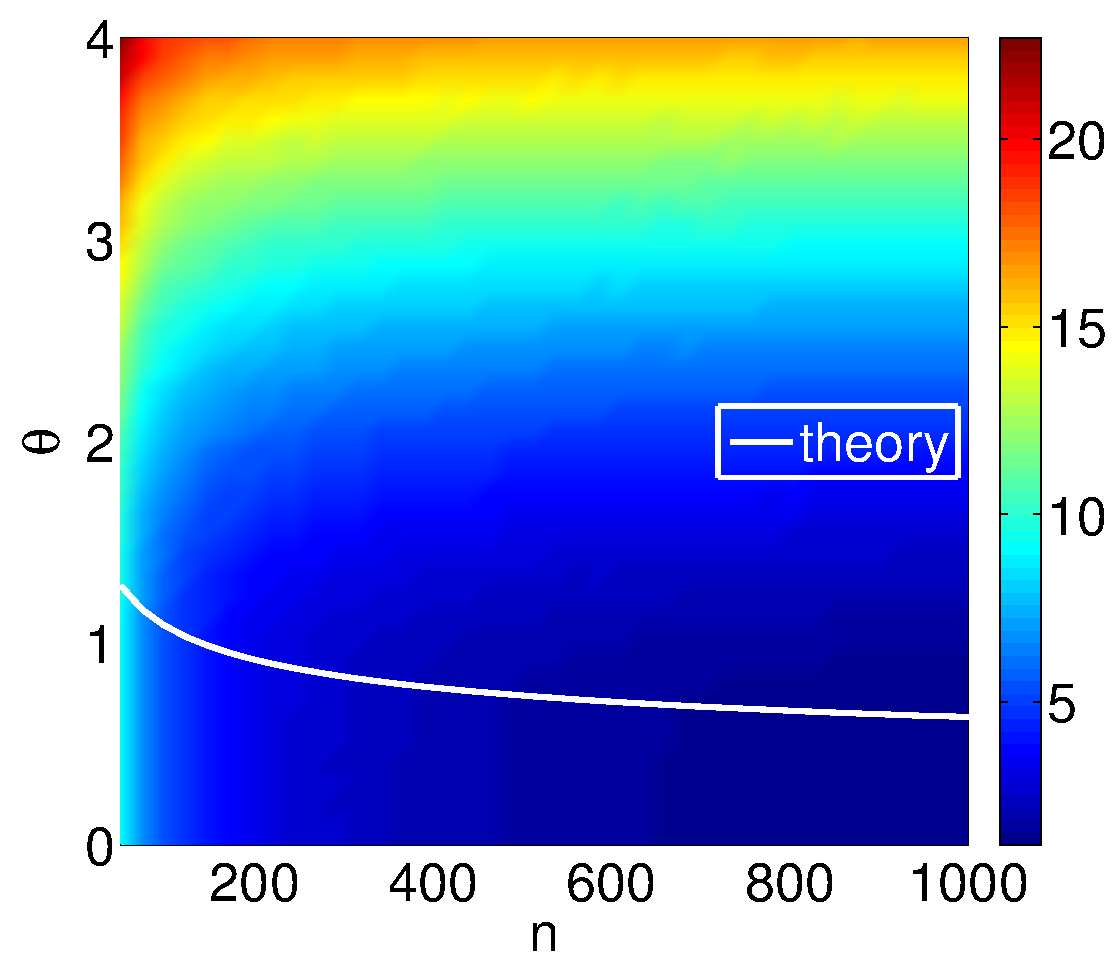
\includegraphics[width=0.4\textwidth]{chpt6_xy/figures/n_theta_large.pdf}
  }
  \subfigure[$\rho=0.1$, $\theta=\theta_{x1}=\theta_{y1}$]{
    \label{fig:chpt6:rcca2}
    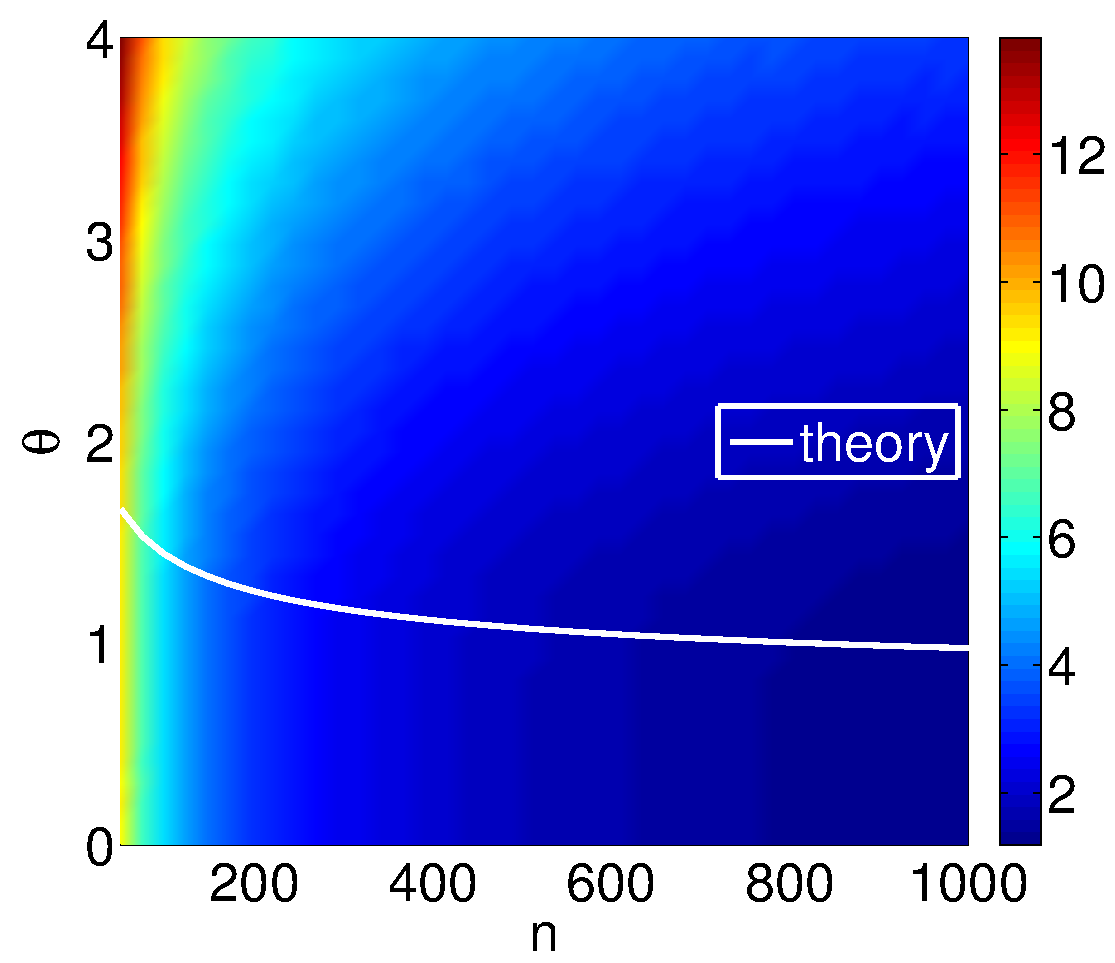
\includegraphics[width=0.4\textwidth]{chpt6_xy/figures/n_theta_small.pdf}
  }
  \subfigure[$\theta_{x1}=\theta_{y1}=1$]{
   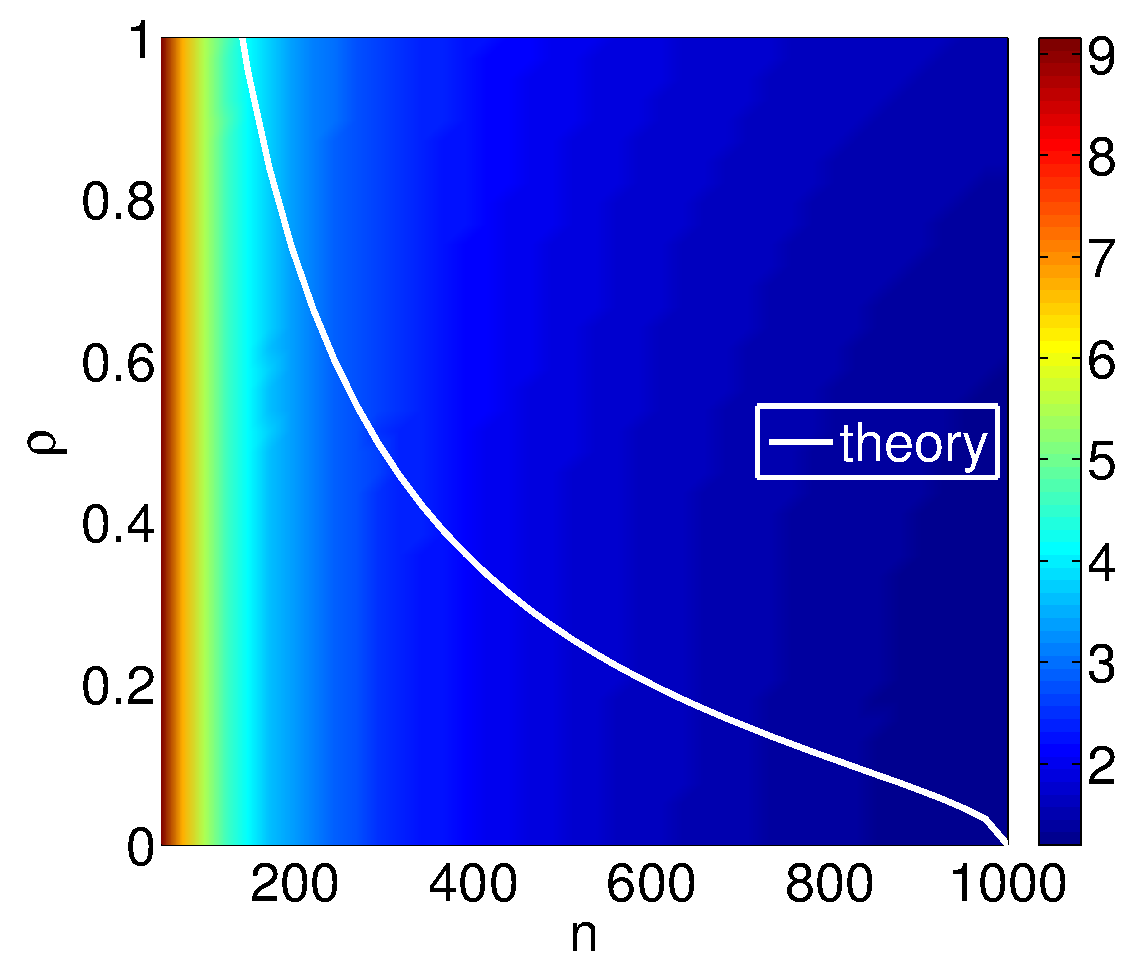
\includegraphics[width=0.4\textwidth]{chpt6_xy/figures/n_rho.pdf}
  }
  \subfigure[$n=400$]{
    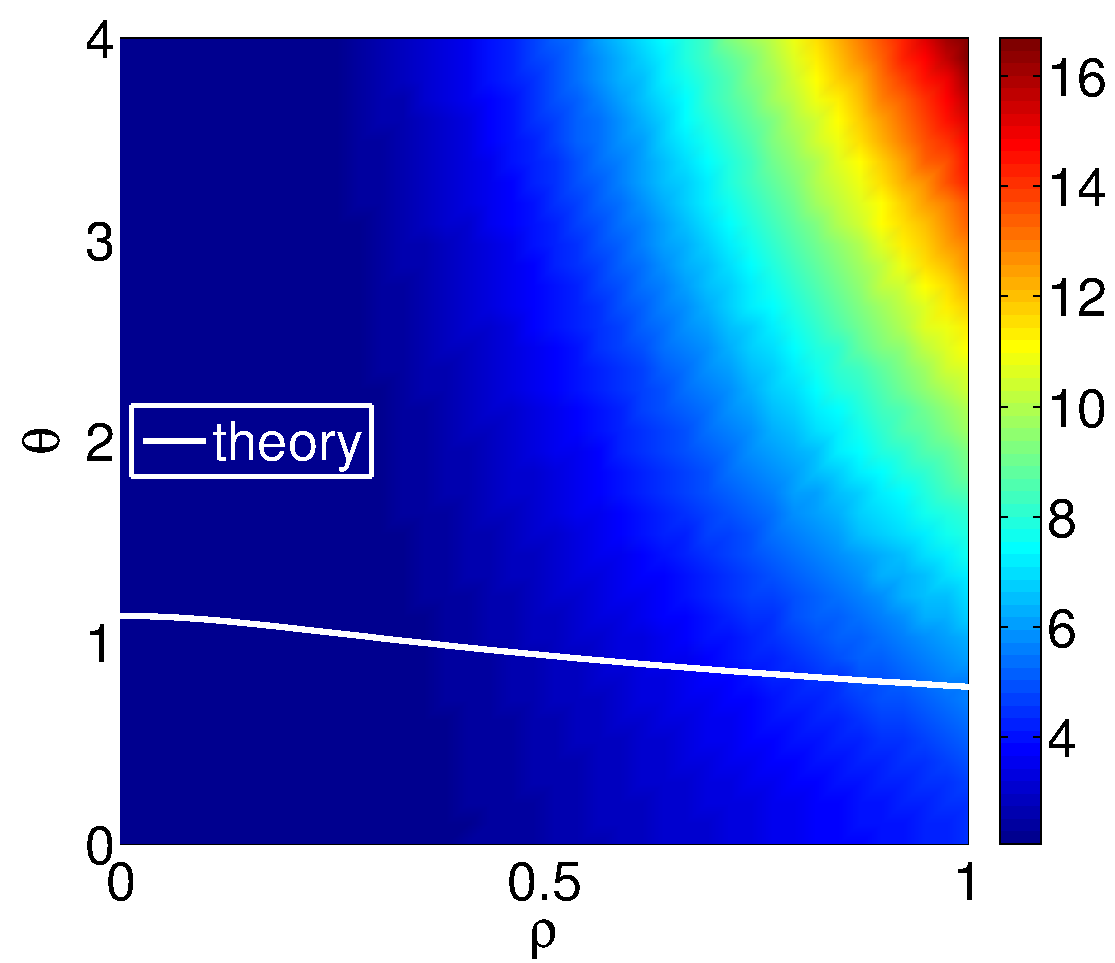
\includegraphics[width=0.4\textwidth]{chpt6_xy/figures/rho_theta.pdf}
  }
  \subfigure[$\rho=0.5$, $n=400$]{
    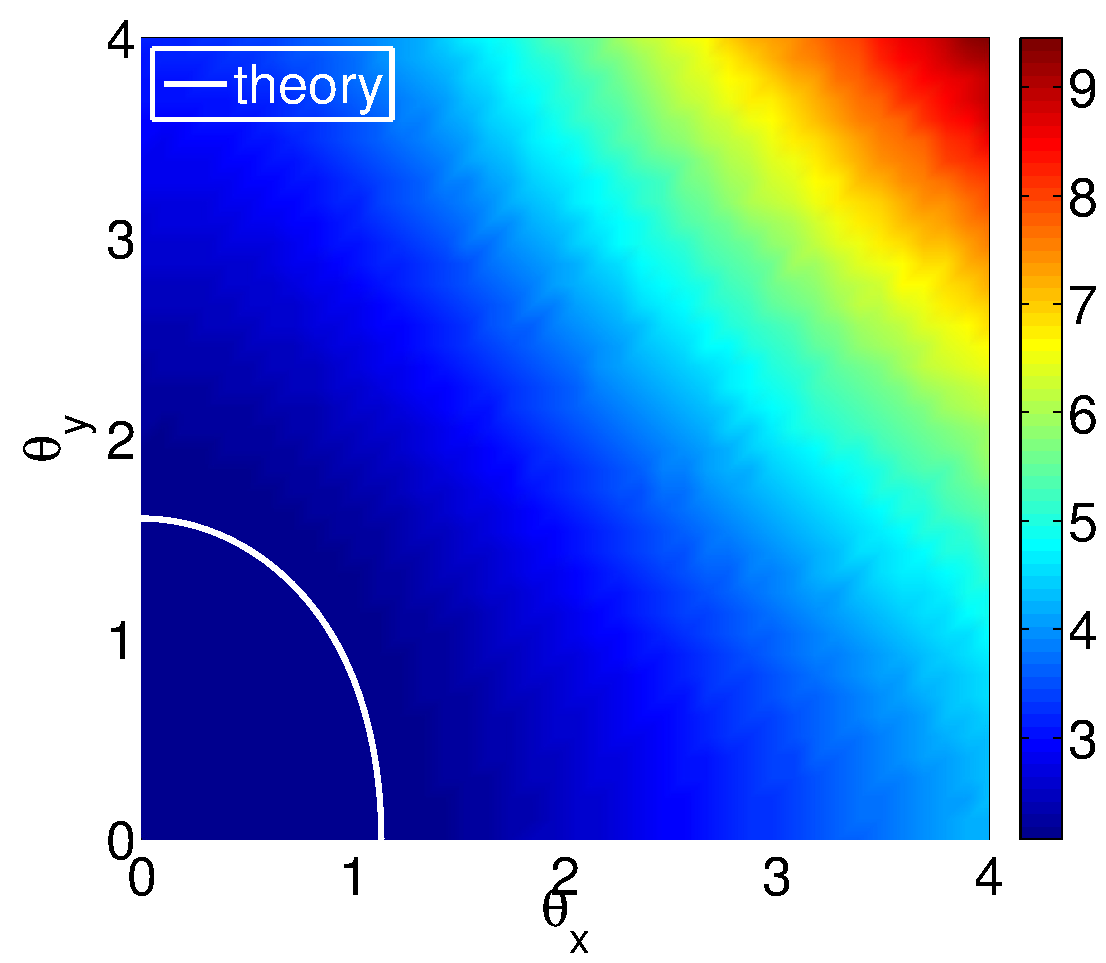
\includegraphics[width=0.4\textwidth]{chpt6_xy/figures/theta_theta.pdf}
    \label{fig:chpt6:theta_theta}
  }
  \caption{Top singular value of LRCCA plotted for pairs of parameter sweeps. In all
    plots, $p=200$ and $q=400$. The theoretical boundary where the top singular value is
    indistinguishable from a noise only setting is plotted for each. Below this line, the
    top singular value is asymptotically identical to the noise only setting. Above this
    line, the top singular value is asymptotically different from that of the noise only
    setting.}
  \label{fig:chpt6:lrcca_pt}
\end{figure}

Next we explore the phase transition in Figure \ref{fig:chpt6:theta_theta} for a fixed $n=400$
and numerous $\rho$. Instead of plotting the top singular value returned by LRCCA, we
instead plot the log of the KS-statistic between the singular values in the signal bearing case
and the singular values in the noise bearing case. A KS statistic of 1 represents
perfectly distinct distributions while a KS statistic of 0 represents the same
distribution. We plot the results in Figure \ref{fig:chpt6:lrcca_ks} and it is evident
that our theoretical phase transition in (\ref{eq:pt}), which relies on Theorem
\ref{thm:xy_sv}, is very accurate even though we apply the asymptotic result to the finite
dimensional setting.  

\begin{figure}[!htbp]
  \centering
  \subfigure[$\rho=1$]{
    \label{fig:chpt6:rcca1}
    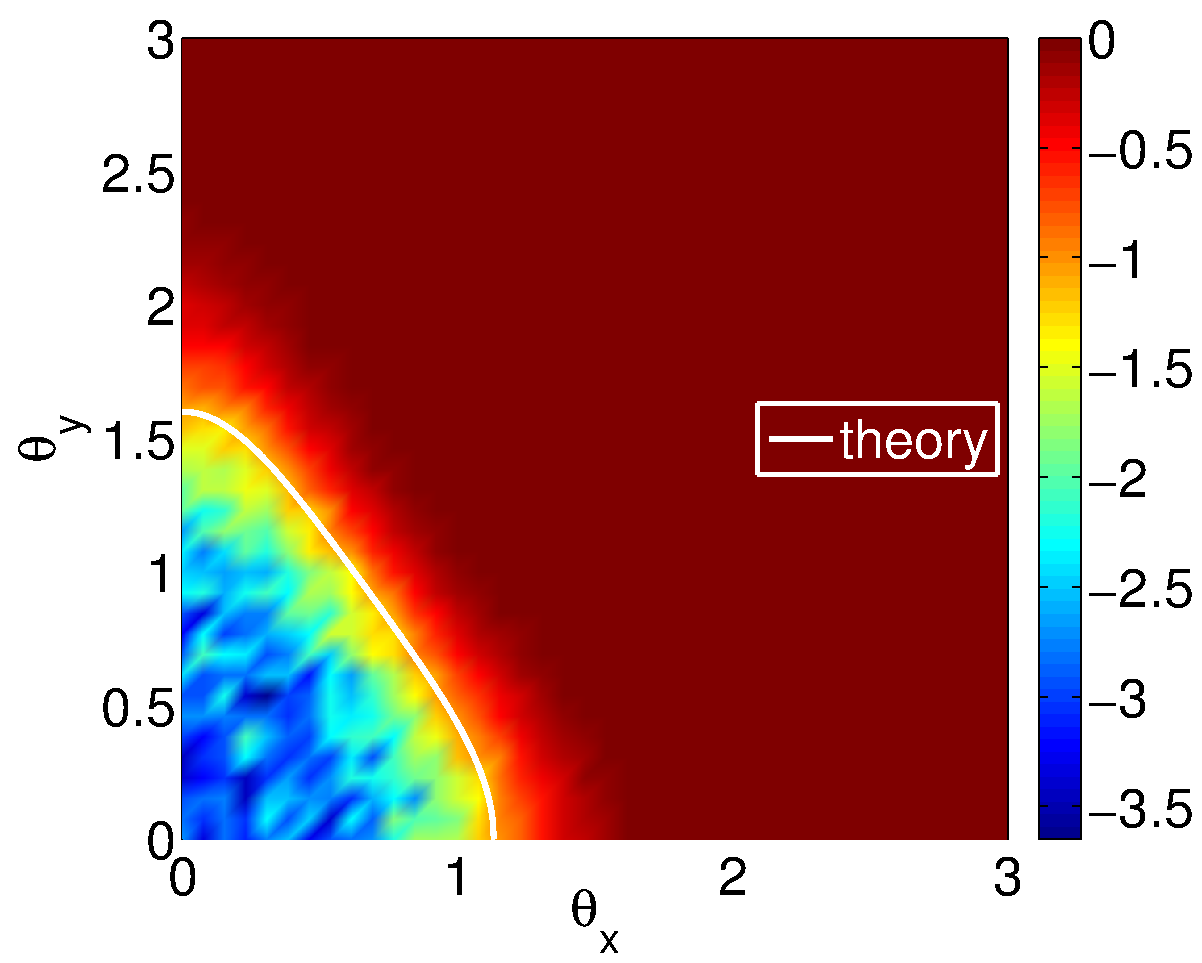
\includegraphics[width=0.4\textwidth]{chpt6_xy/figures/rho_10_theta.pdf}
  }
  \subfigure[$\rho=0.8$]{
    \label{fig:chpt6:rcca2}
    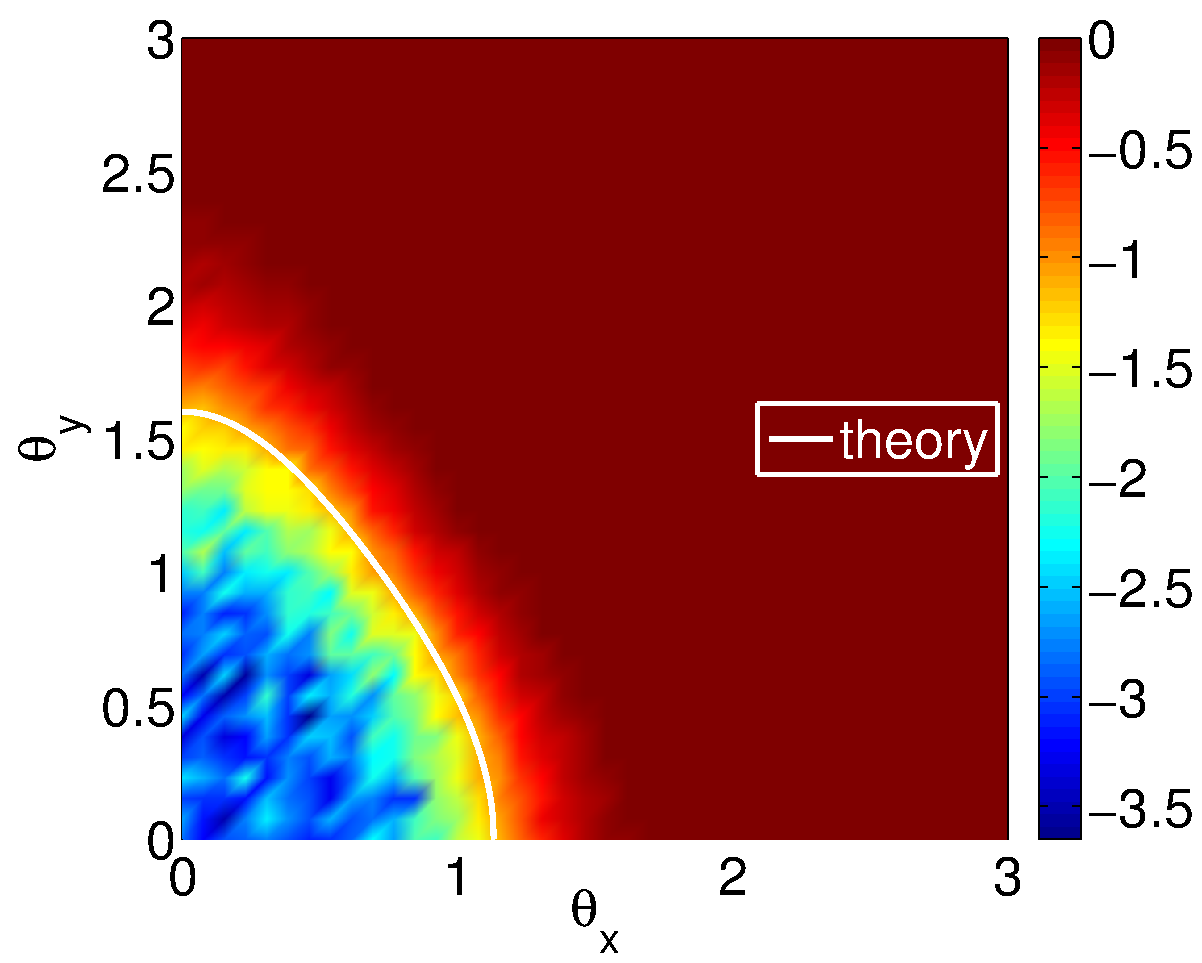
\includegraphics[width=0.4\textwidth]{chpt6_xy/figures/rho_8_theta.pdf}
  }
  \subfigure[$\rho=0.6$]{
   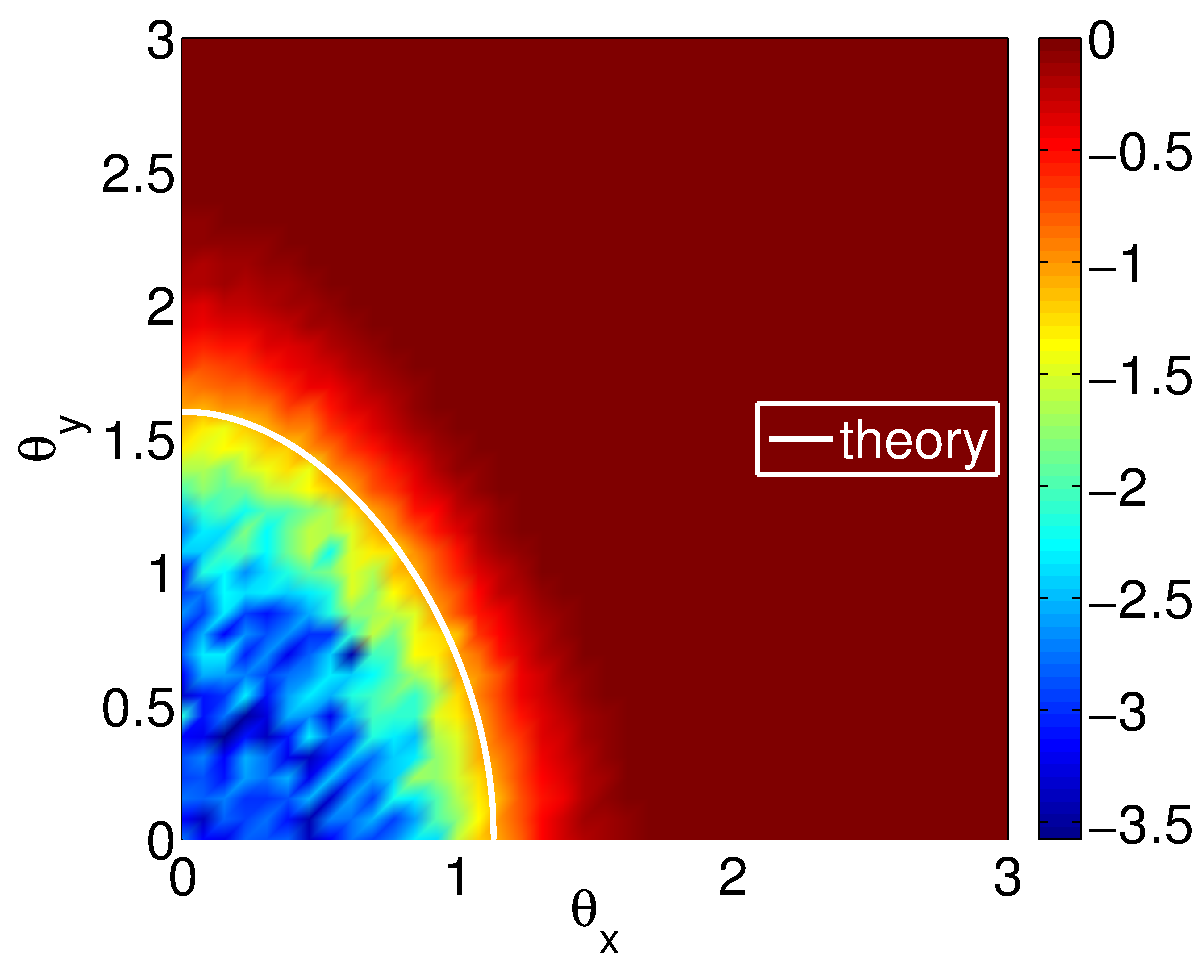
\includegraphics[width=0.4\textwidth]{chpt6_xy/figures/rho_6_theta.pdf}
  }
  \subfigure[$\rho=0.4$]{
    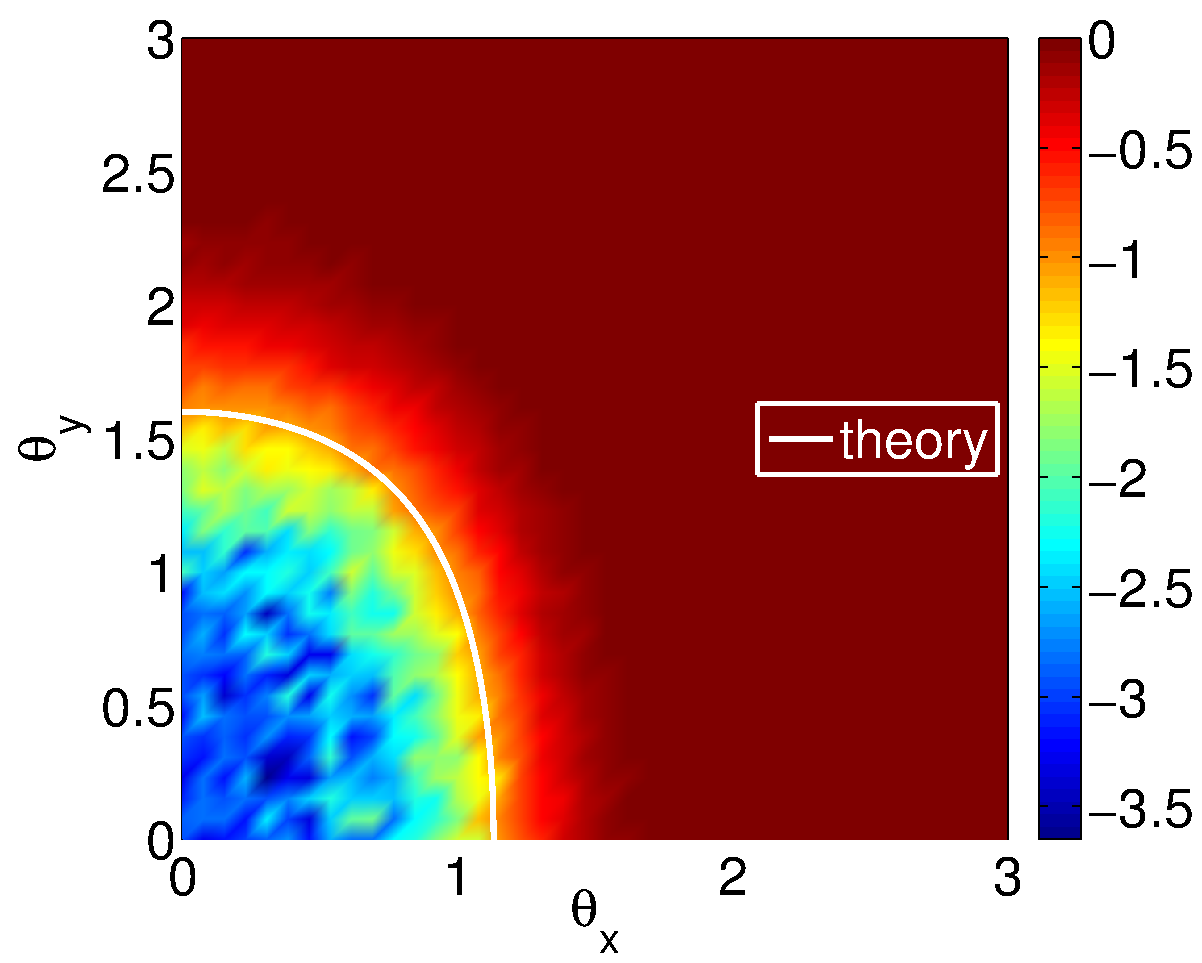
\includegraphics[width=0.4\textwidth]{chpt6_xy/figures/rho_4_theta.pdf}
  }
  \subfigure[$\rho=0.2$]{
    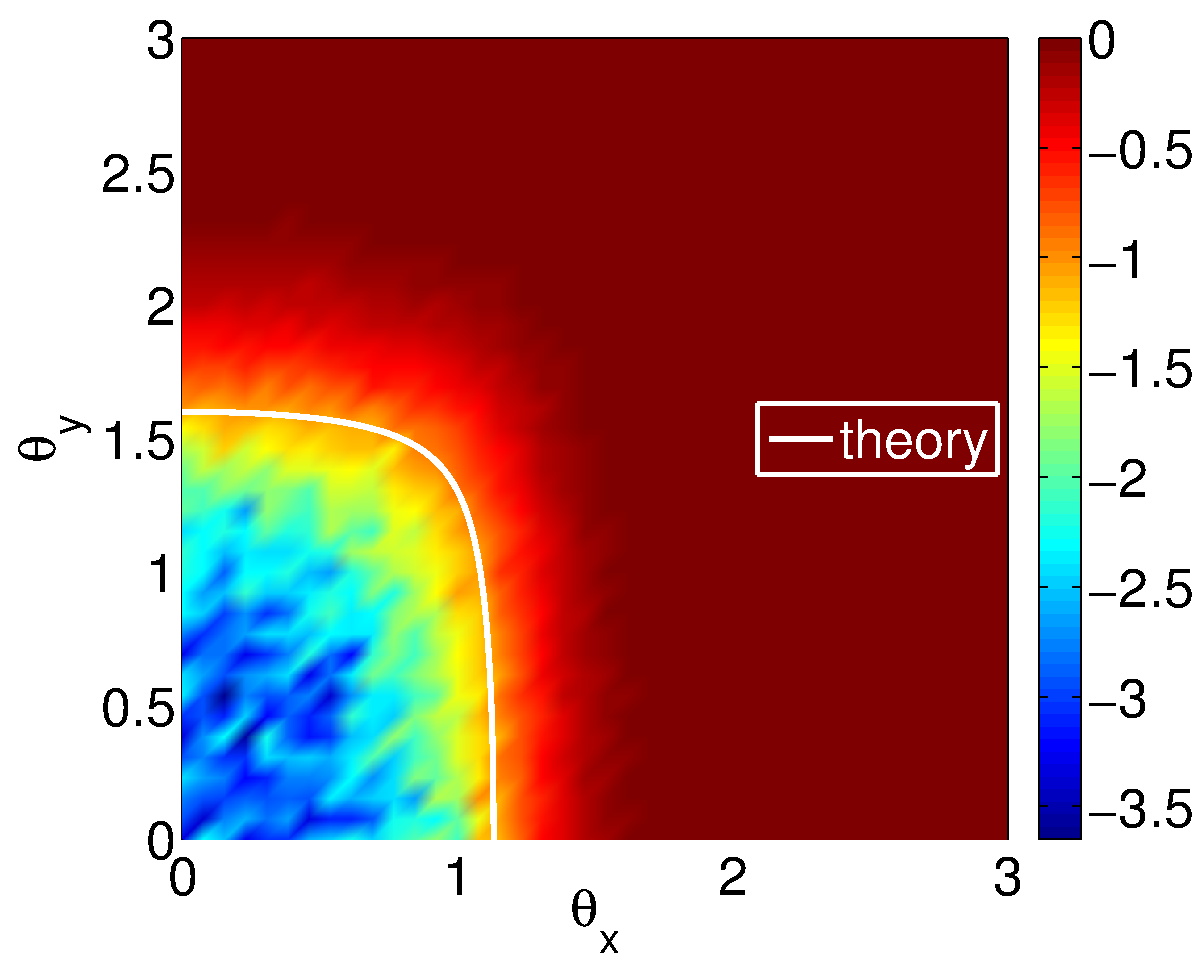
\includegraphics[width=0.4\textwidth]{chpt6_xy/figures/rho_2_theta.pdf}   
  }
  \subfigure[$\rho=0$]{
    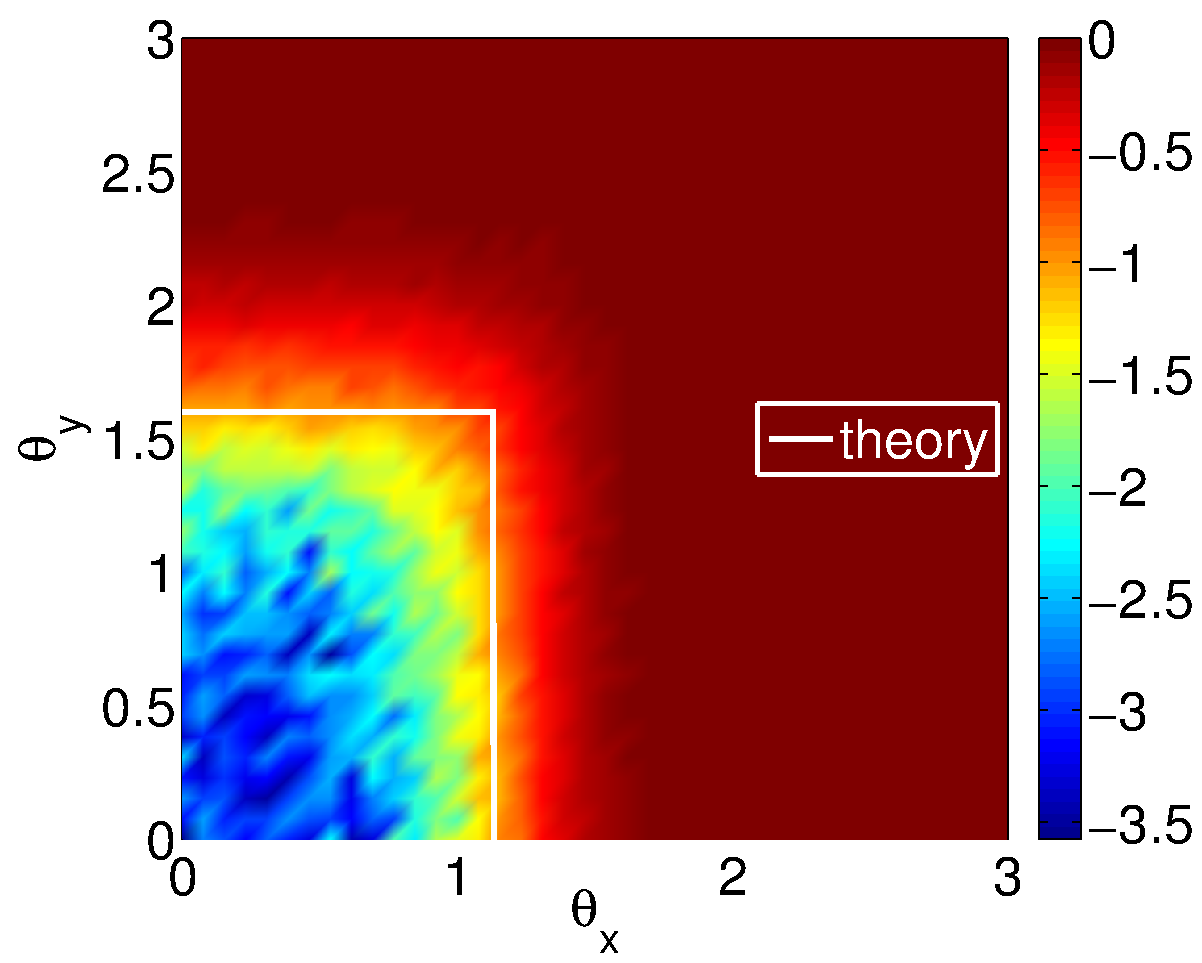
\includegraphics[width=0.4\textwidth]{chpt6_xy/figures/rho_0_theta.pdf}   
  }
  \caption{KS statistic between the top singular value of LRCCA in signal bearing and
    noise only settings. In all plots, $p=200$, $q=400$, and $n=400$. The theoretical boundary where
    the top singular value is indistinguishable from a noise only setting is plotted for
    each.}
  \label{fig:chpt6:lrcca_ks}
\end{figure}

\subsection{Comparison to ICCA}

We now compare the performance of LRCCA to that of ICCA. As shown in
\cite{nadakuditi2011fundamental} and presented in Theorem \ref{th:khat_lims}, the
correlation coefficient does not affect the performance of ICCA. The consistency phase
transition of ICCA for the rank-1 setting is  
\be
\theta_x > c_x^{1/4} \text{ and } \theta_y > c_y^{1/4}.
\ee
We plot this phase transition against the phase transitions of LRCCA for a variety of
$\rho$ in Figure \ref{fig:chpt6:icca_comp}. 

We begin our discussion by comparing what these phase transition boundaries represent for
each algorithm. The ICCA phase transition boundary represents when we reliably detect the
presence of a correlated signal. Above this boundary, the largest singular value of
$\widetilde{C}$ used in ICCA is used to statistically detect the presence of a correlated
signal. We direct the reader to Chapter \ref{sec:chpt_cca_det} for a discussion of this
process. However, if either SNR drops below its individual phase transition, ICCA is not
able to detect a correlated signal. The LRCCA phase transition boundaries, on the other
hand, represent when the largest singular value of $\Clrcca$ represents a signal, not
necessarily a correlated signal. As we saw in Figure \ref{fig:chpt6:motiv_3}, even
uncorrelated datasets will cause the largest singular value to separate from the rest of
the singular value. Therefore, these phase transition boundaries represent different
boundaries. 

One may incorrectly conclude from Figure \ref{fig:chpt6:icca_comp} that for LRCCA is
superior to ICCA since the boundary of LRCCA includes the regime when $\theta_x$ is very
small but $\theta_y$ is large, and vice versa. However, this singular value only indicates
the presence of a signal, not that it is correlated. We saw in Figure
\ref{fig:chpt6:motiv} that different values of $\theta_x,\theta_y,\rho$ can result in the
same largest singular value. Thus, simply using the largest singular value of
$\frac{1}{n}XY^H$ to determine whether correlation exists between the dataset is
incorrect. As Figure \ref{fig:chpt6:motiv_3} shows, the cross covariance matrix will have
a large singular value even if the individual datasets are independent. 

One may then want to use the relative individual SNRs of $X$ and $Y$ to determine whether
this leading singular value is large because of correlation or individual large
SNRs. However, this process of pre-whitening the data matrices $X$ and $Y$ is exactly the
process used in CCA and ICCA. Therefore, to use the cross-covariance matrix $XY^H$ to
detect the presence of correlation between the datasets, one would perform the equivalent
analysis as CCA, which is suboptimal to ICCA. Therefore, we urge users to reconsider using
the cross covariance matrix to screen for correlation and instead use ICCA.

\begin{figure}[!h]
  \begin{center}
    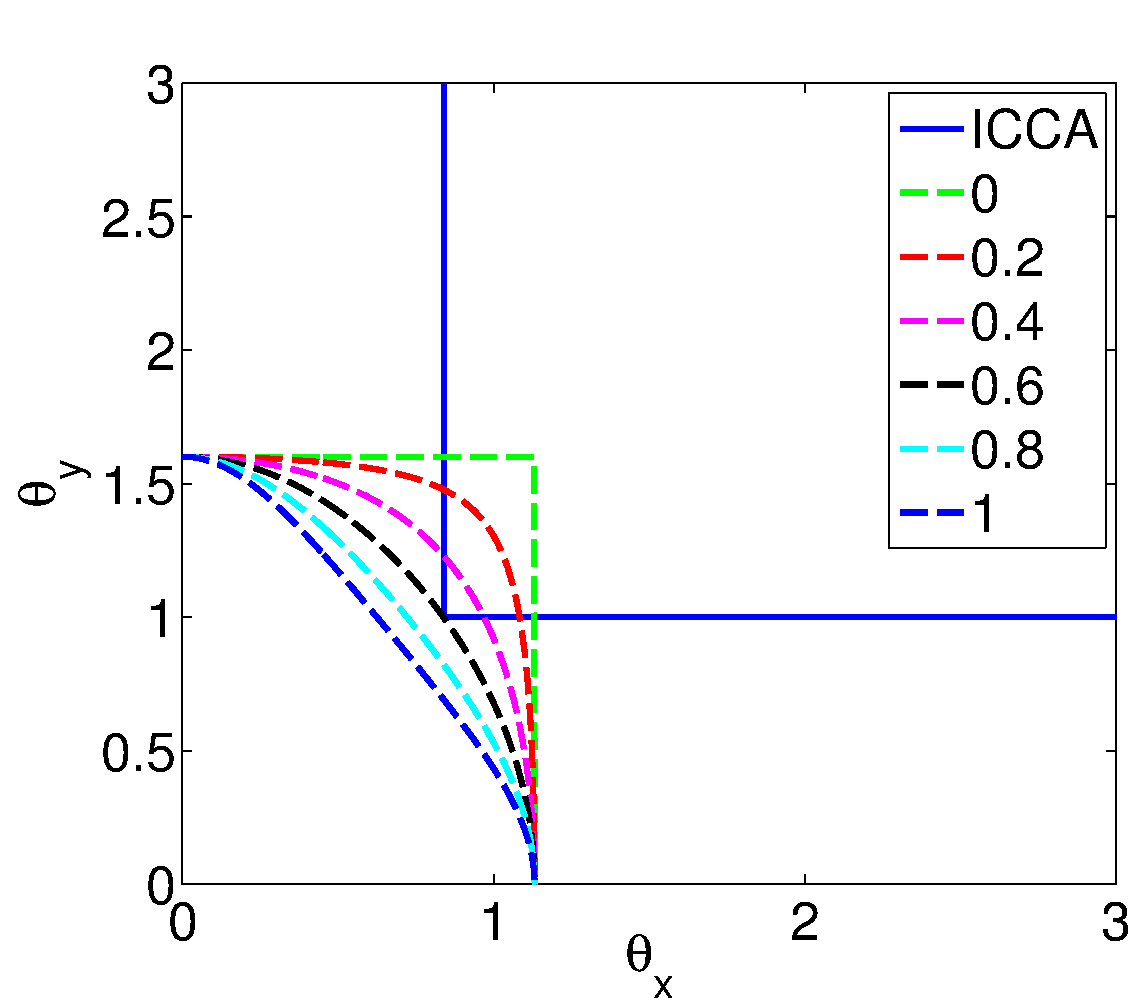
\includegraphics[width=0.6\textwidth]{chpt6_xy/figures/theta_theta_icca.pdf}
    \caption{Phase transition for LRCCA (dahsed lines) for various $\rho$ and ICCA. The
      performance of ICCA is independent of $\rho$. The setting shown in for $c_x=0.5$ and
    $c_y=1$. }
    \label{fig:chpt6:icca_comp}
  \end{center}
\end{figure}

